\begin{solution}

کمترین و بیشترین همبستگی بین $ a $ و $ c $ به ترتیب $-0.5$ و $ 1 $ است.



این یک واقعیت شناخته‌شده است که می‌توان هر توزیع $x$ را به‌ صورت یک بردار $f(x)$ در یک فضای چند بعدی نگاشت کرد به‌طوری که همبستگی دو توزیع $x$ و $y$ برابر با کسینوس زاویه بین $ f(x) $ و $ f(y) $ باشد. توضیحات دقیق‌تری در مورد این موضوع را در انتهای اثبات ارائه می‌دهیم، اما فعلا فرض کنید $ f(a) $، $ f(b) $، و $ f(c) $ بردارهای متناظر برای $ a $، $ b $ و $ c $ با چنین خاصیتی هستند. همبستگی‌ بین $ a $ و هر یک از $ b $ و $ c $ برابر با $ \frac{1}{2} $ است. این به این معناست که زاویه‌ بین $ f(a) $ و هر یک از $ f(b) $ و $ f(c) $ برابر با 60 درجه است. بنابراین، زاویه بین $ f(b) $ و $ f(c) $ می‌تواند هر مقداری بین $-120$ تا $120$ درجه باشد. کمترین کسینوس زاویه‌ها در این بازه $-0.5$ (برای $-120$ و $120$ درجه) و بیشترین کسینوس زاویه‌ها در این بازه $1$ است زمانی که زاویه برابر با 0 درجه باشد.

\begin{center}
	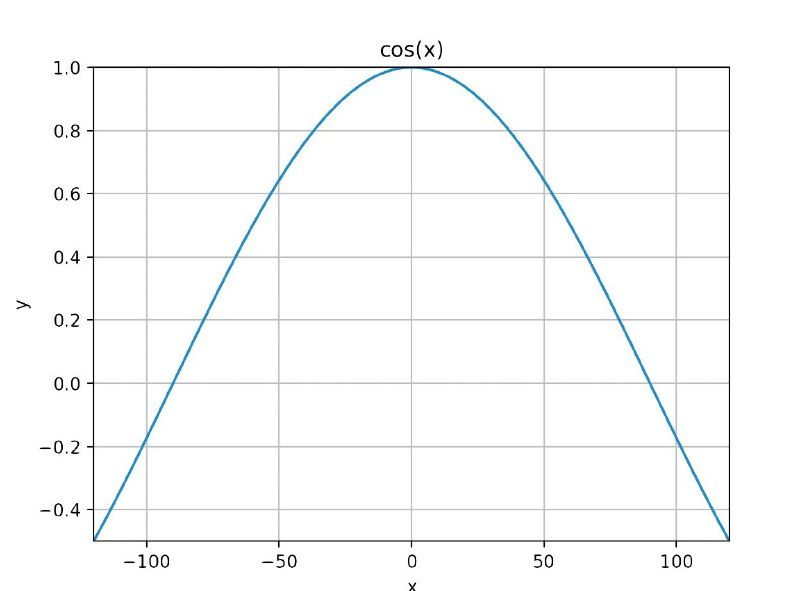
\includegraphics[width=9cm]{/images/problems/81_sol.png}
\end{center}



برای درک رابطه بین توزیع‌ها و بردارها، به تعریف همبستگی توجه کنید:
$$\textsf{cor}(x,y) = \frac{\mathsf{covar}(x,y)}{\sqrt{\mathsf{var}(x)\mathsf{var}(y)}}.$$
فرض کنید $\Omega$ مجموعه‌ای از تمام رویدادهایی است که توزیع‌های احتمالی $x$ و $y$ را تعریف می‌کند و بدون از دست دادن کلیت، فرض کنید که تمام عناصر $\Omega$ احتمال یکسانی دارند. ما $f(x)$ را به‌ شکل یک بردار با ابعاد $|\Omega|$ به‌صورت زیر تعریف می‌کنیم:
$$f(x)_{\omega} = x(\omega) - \bar{x}$$
که در آن $x(\omega)$ مقدار توزیع $x$ برای رویداد $\omega$ و $\bar{x} = \frac{\sum_{\omega' \in \Omega} x(\omega')}{|\Omega|}$ میانگین مقدار توزیع $x$ است. $f(y)$ را نیز به‌ صورت مشابه تعریف می‌کنیم. به این صورت، همبستگی $x$ و $y$ برابر با خواهد بود با:

$$\begin{aligned}
\textsf{cor}(x,y) =& \frac{\mathsf{covar}(x,y)}{\sqrt{\mathsf{var}(x)\mathsf{var}(y)}}\\
= & \frac{\sum_{\omega \in \Omega} (x(\omega) - \bar{x}) (y(\omega) - \bar{y})/|\Omega|}{\sqrt{(\sum_{\omega \in \Omega} (x(\omega) - \bar{x})^2/|\Omega|)(\sum_{\omega \in \Omega} (x(\omega) - \bar{x}))^2/|\Omega|})} \\
= & \frac{\sum_{\omega \in \Omega} (x(\omega) - \bar{x}) (y(\omega) - \bar{y})}{\sqrt{(\sum_{\omega \in \Omega} (x(\omega) - \bar{x}))^2)(\sum_{\omega \in \Omega} (x(\omega) - \bar{x}))^2)}} \\
= & \frac{\sum_{\omega \in \Omega} f(x)_{\omega} f(y)_{\omega}}{\sqrt{(\sum_{\omega \in \Omega} f(x)_{\omega}^2)(\sum_{\omega \in \Omega} f(y)_{\omega}^2)}} \\
= & \frac{\sum_{\omega \in \Omega} f(x)_{\omega} f(y)_{\omega}}{\sqrt{\sum_{\omega \in \Omega} f(x)_{\omega}^2}\sqrt{\sum_{\omega \in \Omega} f(y)_{\omega}^2}} \\
= &  \frac{f(x)\cdot f(y)}{||f(x)|| \cdot ||f(y)||} \\
= & \cos(\textsf{arc}(f(x), f(y)))
\end{aligned} $$

که در آن $\textsf{arc}(f(x), f(y))$ برابر با مقدار زاویه بین $f(x)$ و $f(y)$ است.
\end{solution}
